\section{Calcolo delle portate di progetto (analisi dei deflussi di piena)}
Al fine di conoscere la quantità di deflusso prevista alla sezione di chiusura, occorre prima ricavarsi dei parametri fisici del bacino.

\subsection{Calcolo del tempo di corrivazione del bacino}
Il tempo di corrivazione di un bacino è il tempo che impiega una particella d'acqua ad arrivare alla sezione di chiusura, partendo dal punto idraulicamente più distante da essa.\\
La conoscenza del tempo di corrivazione del bacino permette di prevedere il momento in cui avviene il picco di deflusso alla sezione di chiusura.\\
Esistono diverse metodologie per calcolare il tempo di corrivazione del bacino: metodo cinematico, metodo empirico di Giandotti, di Ferro,...
\subsubsection{Metodo cinematico}
Il metodo cinematico per il calcolo del tempo di corrivazione del bacino implica lo studio del moto dell'acqua sia nel tratto di versante e sia nel tratto di reticolo idrografico.
\begin{equation}
    T_c = T_v + T_r
    \label{tempo_corrivazione}
\end{equation}
Dove:
\begin{itemize}
    \item $T_c$: tempo di corrivazione;
    \item $T_v$: tempo di versante;
    \item $T_r$: tempo di reticolo.
\end{itemize}
Sia per il calcolo del movimento dell'acqua nel reticolo e sia per quello nel versante, è necessario conoscere alcune quote altimetriche del bacino:
\begin{itemize}
    \item $h_0$ (quota della sezione di chiusura): 1183 m s.l.m.;
    \item $h_r$ (quota superiore del collettore principale): 1883 m s.l.m.;
    \item $h_s$ (quota massima del bacino): 2084.3 m s.l.m. 
\end{itemize}
Partendo dalla formula generale della velocità di un fluido: 
\begin{equation}
    V = K_s \cdot R_h^{\frac{2}{3}} \cdot i ^{\frac{1}{2}}
\end{equation}
e svolgendo alcune semplificazioni, è possibile ottenere le formule per il calcolo della velocità nel reticolo e nel versante:
\begin{equation}
    V_R \approx (5 - 10) \cdot i^{\frac{1}{2}}
    \label{vel_reticolo}
\end{equation}
\begin{equation}
    V_v \approx (0.1 - 0.15) i_v^{\frac{1}{2}}
    \label{vel_versante}
\end{equation}
La formula del tempo di corrivazione \ref{tempo_corrivazione} può essere implementata con le formule \ref{vel_versante} e \ref{vel_reticolo}:
\begin{equation}
    T_c = \frac{L_R}{V_R}+ \frac{L_V}{V_V} \approx \frac{L_R}{(5 - 10) \cdot i^{\frac{1}{2}}} + \frac{L_V}{(0.1 - 0.15) i_v^{\frac{1}{2}}}
\end{equation}

Per il calcolo della velocità di reticolo dell'acqua nel bacino, è necessario imporre un valore di pendenza del retico; questo valore si ricava dal rapporto tra la differenza di quota del collettore principale (1883 m-1183 m) e la sua lunghezza (2401 m).\\
Svolgendo la formula \ref{vel_reticolo}, imponendo un coefficiente medio di 7.5, il risultato è $4.05 \frac{m}{s}$.\\
Conoscendo la lunghezza del collettore principale, è possibile ricavare il tempo di corrivazione della componente del reticolo idrografico.\\
In modo analogo, il calcolo della velocità dell'acqua nel versante avviene conoscendo la pendenza del tratto di terreno, ovvero il rapporto tra la differenza di quota (2084.3 m-1883 m) e la sua distanza, ricavata dal GIS, di 445.16 m.\\
Applicando la formula \ref{vel_versante}, applicando un coefficiente di 0.15, la velocità di versante risulta essere di $0.10 \frac{m}{s}$.\\
Anche in questo caso, il tempo di corrivazione nel versante è ricavabile invertendo la formula della velocità.
I tempi di percorrenza dell'acqua sono:
\begin{table}[H] \centering
    \begin{tabular}{ccc}
        \toprule
    \textbf{$T_v$} & \textbf{$T_r$} & {\color[HTML]{000000} } \\
    4413.28     & 592.90      & sec                     \\
    1.23        & 0.16        & ore       \\
    \bottomrule             
    \end{tabular}
    \end{table}
Il tempo di corrivazione totale, ovvero la somma dei due parziali, risulta essere pari a 83.44 minuti (ovvero 1.39 ore).

\subsubsection{Metodo empirico di Giandotti}
Il metodo di Giandotti, per il calcolo del tempo di corrivazione del bacino, richiede l'applicazione della relativa formula:
\begin{equation}
    T_c = \frac{4 \cdot \sqrt{A}+ 1.5 \cdot L}{0.8 \cdot \sqrt{H_m}}
\label{formula_giandotti}
\end{equation}
Dove: 
\begin{itemize}
    \item $T_c$: è il tempo di corrivazione, espresso in ore;
    \item A: è l'area del bacino, espressa in $km^2$;
    \item L: è lunghezza del collettore idraulico, estesa fino allo spartiacque, espressa in km;
    \item $H_m$: è l'altezza media del bacino, riferita alla sezione di chiusura ed espressa in m.
\end{itemize}
Per il bacino in esame:
\begin{itemize}
    \item A: 2.01 $km^2$;
    \item $L_c$: 2.846 $km$;
    \item $H_m$: 470.9 $m$.
\end{itemize}
La formula di Giandotti \ref{formula_giandotti}, con i parametri del bacino in esame, restituisce il tempo di corrivazione di 34.4 minuti (0.573 ore).\\
Questa formula notoriamente restituisce valori di corrivazione molto contenuti rispetto a quelli reali.

\subsubsection{Metodo empirico di Ferro (I)}
La formula necessaria da applicare per questo metodo è la seguente:
\begin{equation}
    T_c = 0.022 \cdot \left(\frac{L_C}{i^{0.5}}\right)^{0.8}
    \label{formula_ferro_I}
\end{equation}
Dove: 
\begin{itemize}
    \item $T_c$: viene espressa in minuti;
    \item $L_C$: viene espressa in metri;
    \item i: viene espressa $\frac{m}{m}$.
\end{itemize}
Nel caso del bacino in esame:
\begin{itemize}
    \item A: 2.01 $km^2$;
    \item $L_C$: 2401 $m$;
    \item $i_r$: 0.293 $\frac{m}{m}$.
\end{itemize}
La formula del metodo di Ferro (I) \ref{formula_ferro_I} restituisce il valore di 18.19 minuti.\\
Nel caso di bacini montani con collettore principale corto (qualche chilometro), e ripido, la formula tende a sottostimare il valore reale.

\subsubsection{Metodo empirico di Ferro (II)}
La formula di Ferro (II) richiede solamente la conoscenza dell'area del bacino:
\begin{equation}
    T_c = 0.675 \cdot \sqrt{A}
    \label{formula_ferro_II}
\end{equation}
Dove:
\begin{itemize}
    \item $T_c$: viene espressa in ore;
    \item $A$: viene espressa in $km^2$.
\end{itemize}
Nel caso del nostro bacino, come già riportato prima, l'area è pari a 2.01 $km^2$.\\
La formula \ref{formula_ferro_II} restituisce un tempo di corrivazione pari a 57.42 minuti (0.96 ore).

\subsection{Comparazione dei metodi di corrivazione}
Dopo aver applicato diversi metodi per il calcolo del tempo di corrivazione, risulta utile compararli.
\begin{table}[H] \centering
    \caption{\textcolor{red}{Comparazione dei diversi metodi di calcolo del tempo di corrivazione.}}
    \begin{tabular}{ccc}
        \toprule
  Metodo di calcolo   & $T_c$ in minuti & $T_c$ in ore\\
     \midrule
   Cinematico  & 83.44 & 1.39\\
   Giandotti  & 34.356 & 0.573\\
   Ferro (I)  & 18.19 & 0.30\\
   Ferro (II)  &57.42 & 0.96\\
     \bottomrule
    \end{tabular}
    \end{table}
A seconda del caso di studio o di lavoro in esame, ogni metodo di calcolo trova la propria migliore applicazione.\\
Ovviamente, conoscendo le distanze dei tratti (di reticolo e di versante) e le relative velocità dell'acqua in movimento, il metodo cinematico risulta quello che calcola nel modo più affidabile possibile il tempo di corrivazione del bacino. Lo stesso ragionamento può essere svolto considerando che tale metodo è l'unico fisicamente basato tra tutti quelli elencati. Per tali motivi, verrà utilizzato questo risultato per le successive valutazioni inerenti ai calcoli dei deflussi attesi.\\
Nei casi in cui, per questioni di tempo o per mancanza di dati, il metodo cinematico non fosse utilizzabile, l'applicazione degli altri metodi per il calcolo del tempo di corrivazione dev'essere svolta considerando l'assunzione di inevitabili errori. 

\subsection{Determinazione del parametro idrologico CN}
Al fine di descrivere la tendenza di un suolo a generare runoff o infiltrazione sottosuperficiale (a fronte di un evento pluviometrico), il dipartimento di agricoltura americano (USDA) ha idealizzato il metodo SCS-CN (\textit{soil conservation service - curve number}).\\
In seguito ad analisi empiriche, ad ogni tipologia di suolo e soprassuolo sono associati precisi valori, in una scala che va da 0 a 100.\\
Maggiore è il valore attribuito all'area e maggiore è la tendenza che si crei deflusso superficiale. Viceversa, minore è il numero dell'indice e maggiore sarà la capacità del suolo ad infiltrare acqua. I valori CN sono generalmente tabellati, e rilasciati da vari enti pubblici (\ref{scs_cn_table}).\\
La qualità litologica del suolo viene descritta secondo 4 gruppi (dalla A alla D), con capacità di infiltrazione dell'acqua sempre minore.\\

\begin{figure}[H]  \centering
    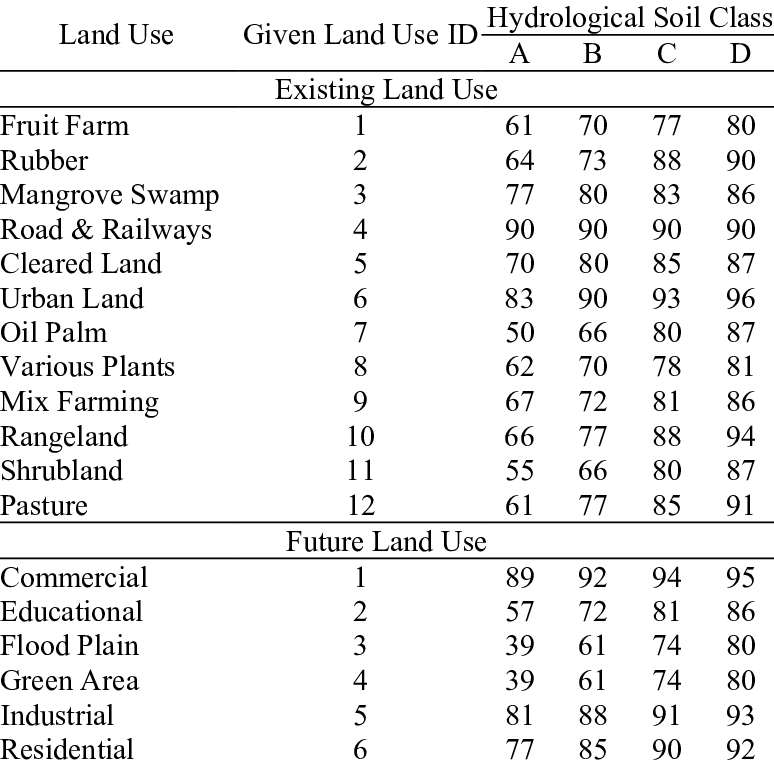
\includegraphics[scale=0.5]{immagini/scs_cn_table.png}
    \caption{Valori tabellari del parametro idrologico CN.}
    \label{scs_cn_table}
\end{figure}

Il parametro CN, oltre che essere dipendente dalla natura del suolo o dall'utilizzo del soprassuolo, viene influenzato anche dalle condizioni pluviometriche incidenti nei giorni precedenti del momento di studio.\\
Generalmente, tutti i valori tabellati, a meno che non venga specificato, si trovano in condizione AMC (\textit{Antecedent Moisture Conditions}) numero II, ovvero in grado medio.\\
I parametri AMC vengono imposti considerando le seguenti condizioni:
\begin{figure}[H]  \centering
    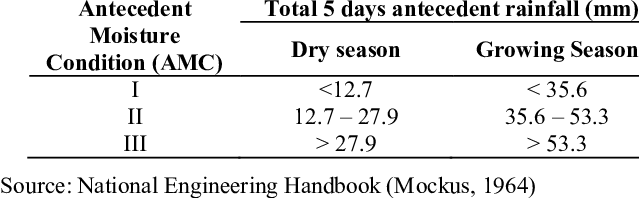
\includegraphics[scale=0.7]{immagini/AMC_table.png}
    \caption{Condizioni idrologiche del suolo antecedenti l'evento di pioggia AMC (I), AMC (II) e AMC (III).}
    \label{AMC_table}
\end{figure}
Le trasformazioni tra le diverse condizioni avvengono mediante le formule:
\begin{equation}
    AMC (I)\rightarrow CN (I) = \frac{4.2 \cdot CN(II)}{10-0.058 \cdot CN(II)}
\end{equation}
\begin{equation}
    AMC(III) \rightarrow CN(III) = \frac{23\cdot CN (II)}{10+0.13 \cdot CN(II)}
\end{equation}
La condizione più favorevole, ovvero la AMC (III), è quella che genera il maggior deflusso, e che è quindi preferibile da utilizzare in sede di progetto.\\
Il limite di saturazione dell'acqua nel terreno (S), ovvero la massima quantità infiltrabile, viene ricavata dal parametro CN del suolo-soprassuolo, utilizzando la formula:
\begin{equation}
    S = 25.4 \cdot \left(\frac{1000}{CN} -10 \right)
\end{equation} 
Al fine di conoscere le quantità di pioggia che si trasformano in deflusso, che vengono intercettate o che vengono assorbite, viene applicata la formula $P_e = \frac{(P-I_a)^2}{P-I_a+S} \label{eq_PE}$, che derivano dalle seguenti:
\begin{figure}[H]
\begin{equation}
    \frac{P_e}{P-I_a} = \frac{F_a}{S} 
\end{equation}
\caption*{Relazione empirica che lega le diverse componenti dell'acqua meteorica in arrivo.}
\end{figure}
\begin{figure}[H]
\begin{equation}
    P= P_e + I_a + F_a     
\end{equation}
\caption*{Equazione di continuità.}
\end{figure}

Nell'equazione \ref{eq_PE}, oltre ad essere presenti i valori di pioggia in arrivo (P) e di storage idrico del terreno (S), viene considerato anche il parametro riguardante la perdita iniziale di acqua ($I_a$).\\
Tale valore è dipendente da S, e varia da 0 a $0.2\cdot S$; riguarda tutto il volume di pioggia intercetta dalla vegetazione, o dalle cavità nel terreno, che non si infiltra e che non diventa deflusso.